\begin{tikzpicture}
\pgfdeclareplotmark{cross} {
\pgfpathmoveto{\pgfpoint{-0.3\pgfplotmarksize}{\pgfplotmarksize}}
\pgfpathlineto{\pgfpoint{+0.3\pgfplotmarksize}{\pgfplotmarksize}}
\pgfpathlineto{\pgfpoint{+0.3\pgfplotmarksize}{0.3\pgfplotmarksize}}
\pgfpathlineto{\pgfpoint{+1\pgfplotmarksize}{0.3\pgfplotmarksize}}
\pgfpathlineto{\pgfpoint{+1\pgfplotmarksize}{-0.3\pgfplotmarksize}}
\pgfpathlineto{\pgfpoint{+0.3\pgfplotmarksize}{-0.3\pgfplotmarksize}}
\pgfpathlineto{\pgfpoint{+0.3\pgfplotmarksize}{-1.\pgfplotmarksize}}
\pgfpathlineto{\pgfpoint{-0.3\pgfplotmarksize}{-1.\pgfplotmarksize}}
\pgfpathlineto{\pgfpoint{-0.3\pgfplotmarksize}{-0.3\pgfplotmarksize}}
\pgfpathlineto{\pgfpoint{-1.\pgfplotmarksize}{-0.3\pgfplotmarksize}}
\pgfpathlineto{\pgfpoint{-1.\pgfplotmarksize}{0.3\pgfplotmarksize}}
\pgfpathlineto{\pgfpoint{-0.3\pgfplotmarksize}{0.3\pgfplotmarksize}}
\pgfpathclose
\pgfusepathqstroke
}
\pgfdeclareplotmark{cross*} {
\pgfpathmoveto{\pgfpoint{-0.3\pgfplotmarksize}{\pgfplotmarksize}}
\pgfpathlineto{\pgfpoint{+0.3\pgfplotmarksize}{\pgfplotmarksize}}
\pgfpathlineto{\pgfpoint{+0.3\pgfplotmarksize}{0.3\pgfplotmarksize}}
\pgfpathlineto{\pgfpoint{+1\pgfplotmarksize}{0.3\pgfplotmarksize}}
\pgfpathlineto{\pgfpoint{+1\pgfplotmarksize}{-0.3\pgfplotmarksize}}
\pgfpathlineto{\pgfpoint{+0.3\pgfplotmarksize}{-0.3\pgfplotmarksize}}
\pgfpathlineto{\pgfpoint{+0.3\pgfplotmarksize}{-1.\pgfplotmarksize}}
\pgfpathlineto{\pgfpoint{-0.3\pgfplotmarksize}{-1.\pgfplotmarksize}}
\pgfpathlineto{\pgfpoint{-0.3\pgfplotmarksize}{-0.3\pgfplotmarksize}}
\pgfpathlineto{\pgfpoint{-1.\pgfplotmarksize}{-0.3\pgfplotmarksize}}
\pgfpathlineto{\pgfpoint{-1.\pgfplotmarksize}{0.3\pgfplotmarksize}}
\pgfpathlineto{\pgfpoint{-0.3\pgfplotmarksize}{0.3\pgfplotmarksize}}
\pgfpathclose
\pgfusepathqfillstroke
}
\pgfdeclareplotmark{newstar} {
\pgfpathmoveto{\pgfqpoint{0pt}{\pgfplotmarksize}}
\pgfpathlineto{\pgfqpointpolar{44}{0.5\pgfplotmarksize}}
\pgfpathlineto{\pgfqpointpolar{18}{\pgfplotmarksize}}
\pgfpathlineto{\pgfqpointpolar{-20}{0.5\pgfplotmarksize}}
\pgfpathlineto{\pgfqpointpolar{-54}{\pgfplotmarksize}}
\pgfpathlineto{\pgfqpointpolar{-90}{0.5\pgfplotmarksize}}
\pgfpathlineto{\pgfqpointpolar{234}{\pgfplotmarksize}}
\pgfpathlineto{\pgfqpointpolar{198}{0.5\pgfplotmarksize}}
\pgfpathlineto{\pgfqpointpolar{162}{\pgfplotmarksize}}
\pgfpathlineto{\pgfqpointpolar{134}{0.5\pgfplotmarksize}}
\pgfpathclose
\pgfusepathqstroke
}
\pgfdeclareplotmark{newstar*} {
\pgfpathmoveto{\pgfqpoint{0pt}{\pgfplotmarksize}}
\pgfpathlineto{\pgfqpointpolar{44}{0.5\pgfplotmarksize}}
\pgfpathlineto{\pgfqpointpolar{18}{\pgfplotmarksize}}
\pgfpathlineto{\pgfqpointpolar{-20}{0.5\pgfplotmarksize}}
\pgfpathlineto{\pgfqpointpolar{-54}{\pgfplotmarksize}}
\pgfpathlineto{\pgfqpointpolar{-90}{0.5\pgfplotmarksize}}
\pgfpathlineto{\pgfqpointpolar{234}{\pgfplotmarksize}}
\pgfpathlineto{\pgfqpointpolar{198}{0.5\pgfplotmarksize}}
\pgfpathlineto{\pgfqpointpolar{162}{\pgfplotmarksize}}
\pgfpathlineto{\pgfqpointpolar{134}{0.5\pgfplotmarksize}}
\pgfpathclose
\pgfusepathqfillstroke
}
\definecolor{c}{rgb}{1,1,1};
\draw [color=c, fill=c] (0,0) rectangle (20,14.4361);
\draw [color=c, fill=c] (2,1.44361) rectangle (18,12.9925);
\definecolor{c}{rgb}{0,0,0};
\draw [c,line width=0.9] (2,1.44361) -- (2,12.9925) -- (18,12.9925) -- (18,1.44361) -- (2,1.44361);
\definecolor{c}{rgb}{0.482353,0.670588,0.894118};
\draw [color=c, fill=c] (2,1.44361) rectangle (5.37553,3.60902);
\draw [color=c, fill=c] (5.37553,1.44361) rectangle (8.75105,3.60902);
\definecolor{c}{rgb}{0.600245,0.798039,0.875};
\draw [color=c, fill=c] (8.75105,1.44361) rectangle (11.2489,3.60902);
\definecolor{c}{rgb}{0.823529,0.905882,0.823529};
\draw [color=c, fill=c] (12.2616,1.44361) rectangle (15.5021,3.60902);
\definecolor{c}{rgb}{0.817157,0.659804,0.345588};
\draw [color=c, fill=c] (15.5021,1.44361) rectangle (18,3.60902);
\definecolor{c}{rgb}{0.482353,0.670588,0.894118};
\draw [color=c, fill=c] (2,3.60902) rectangle (5.37553,5.05263);
\draw [color=c, fill=c] (5.37553,3.60902) rectangle (8.75105,5.05263);
\definecolor{c}{rgb}{0.600245,0.798039,0.875};
\draw [color=c, fill=c] (8.75105,3.60902) rectangle (11.2489,5.05263);
\definecolor{c}{rgb}{0.860294,0.872181,0.670343};
\draw [color=c, fill=c] (12.2616,3.60902) rectangle (15.5021,5.05263);
\definecolor{c}{rgb}{0.719608,0.263113,0.13652};
\draw [color=c, fill=c] (15.5021,3.60902) rectangle (18,5.05263);
\definecolor{c}{rgb}{0.482353,0.670588,0.894118};
\draw [color=c, fill=c] (2,5.05263) rectangle (5.37553,7.21805);
\draw [color=c, fill=c] (5.37553,5.05263) rectangle (8.75105,7.21805);
\definecolor{c}{rgb}{0.600245,0.798039,0.875};
\draw [color=c, fill=c] (8.75105,5.05263) rectangle (11.2489,7.21805);
\definecolor{c}{rgb}{0.860294,0.872181,0.670343};
\draw [color=c, fill=c] (12.2616,5.05263) rectangle (15.5021,7.21805);
\definecolor{c}{rgb}{0.719608,0.263113,0.13652};
\draw [color=c, fill=c] (15.5021,5.05263) rectangle (18,7.21805);
\definecolor{c}{rgb}{0.482353,0.670588,0.894118};
\draw [color=c, fill=c] (2,7.21805) rectangle (5.37553,12.9925);
\draw [color=c, fill=c] (5.37553,7.21805) rectangle (8.75105,12.9925);
\definecolor{c}{rgb}{0.600245,0.798039,0.875};
\draw [color=c, fill=c] (8.75105,7.21805) rectangle (11.2489,12.9925);
\definecolor{c}{rgb}{0.842647,0.888358,0.743873};
\draw [color=c, fill=c] (12.2616,7.21805) rectangle (15.5021,12.9925);
\definecolor{c}{rgb}{0.719608,0.263113,0.13652};
\draw [color=c, fill=c] (15.5021,7.21805) rectangle (18,12.9925);
\definecolor{c}{rgb}{0,0,0};
\draw (3.68776,2.52632) node[scale=1.61424, color=c, rotate=1]{$\genfrac{}{}{0pt}{}{2.568}{\pm 0.004}$};
\draw (7.06329,2.52632) node[scale=1.61424, color=c, rotate=1]{$\genfrac{}{}{0pt}{}{2.747}{\pm 0.008}$};
\draw (10,2.52632) node[scale=1.61424, color=c, rotate=1]{$\genfrac{}{}{0pt}{}{4.044}{\pm 0.023}$};
\draw (13.8819,2.52632) node[scale=1.61424, color=c, rotate=1]{$\genfrac{}{}{0pt}{}{5.483}{\pm 0.060}$};
\draw (16.7511,2.52632) node[scale=1.61424, color=c, rotate=1]{$\genfrac{}{}{0pt}{}{8.839}{\pm 0.109}$};
\draw (3.68776,4.33083) node[scale=1.61424, color=c, rotate=1]{$\genfrac{}{}{0pt}{}{2.712}{\pm 0.026}$};
\draw (7.06329,4.33083) node[scale=1.61424, color=c, rotate=1]{$\genfrac{}{}{0pt}{}{2.551}{\pm 0.022}$};
\draw (10,4.33083) node[scale=1.61424, color=c, rotate=1]{$\genfrac{}{}{0pt}{}{3.708}{\pm 0.017}$};
\draw (13.8819,4.33083) node[scale=1.61424, color=c, rotate=1]{$\genfrac{}{}{0pt}{}{6.413}{\pm 0.029}$};
\draw (16.7511,4.33083) node[scale=1.61424, color=c, rotate=1]{$\genfrac{}{}{0pt}{}{11.154}{\pm 0.026}$};
\draw (3.68776,6.13534) node[scale=1.61424, color=c, rotate=1]{$\genfrac{}{}{0pt}{}{2.669}{\pm 0.014}$};
\draw (7.06329,6.13534) node[scale=1.61424, color=c, rotate=1]{$\genfrac{}{}{0pt}{}{2.523}{\pm 0.016}$};
\draw (10,6.13534) node[scale=1.61424, color=c, rotate=1]{$\genfrac{}{}{0pt}{}{3.812}{\pm 0.044}$};
\draw (13.8819,6.13534) node[scale=1.61424, color=c, rotate=1]{$\genfrac{}{}{0pt}{}{6.437}{\pm 0.024}$};
\draw (16.7511,6.13534) node[scale=1.61424, color=c, rotate=1]{$\genfrac{}{}{0pt}{}{11.629}{\pm 0.054}$};
\draw (3.68776,10.1053) node[scale=1.61424, color=c, rotate=1]{$\genfrac{}{}{0pt}{}{2.576}{\pm 0.042}$};
\draw (7.06329,10.1053) node[scale=1.61424, color=c, rotate=1]{$\genfrac{}{}{0pt}{}{2.523}{\pm 0.040}$};
\draw (10,10.1053) node[scale=1.61424, color=c, rotate=1]{$\genfrac{}{}{0pt}{}{3.798}{\pm 0.063}$};
\draw (13.8819,10.1053) node[scale=1.61424, color=c, rotate=1]{$\genfrac{}{}{0pt}{}{6.347}{\pm 0.118}$};
\draw (16.7511,10.1053) node[scale=1.61424, color=c, rotate=1]{$\genfrac{}{}{0pt}{}{11.358}{\pm 0.175}$};
\draw [c,line width=0.9] (2,1.44361) -- (18,1.44361);
\draw [anchor=north] (3.68776,1.27038) node[scale=0.723624, color=c, rotate=0]{[0.0 - 0.5]};
\draw [anchor=north] (7.06329,1.27038) node[scale=0.723624, color=c, rotate=0]{[0.5 - 1.0]};
\draw [anchor=north] (10,1.27038) node[scale=0.723624, color=c, rotate=0]{[1.0 - 1.37]};
\draw [anchor=north] (11.7553,1.27038) node[scale=0.723624, color=c, rotate=0]{[1.37 - 1.52]};
\draw [anchor=north] (13.8819,1.27038) node[scale=0.723624, color=c, rotate=0]{[1.52 - 2.0]};
\draw [anchor=north] (16.7511,1.27038) node[scale=0.723624, color=c, rotate=0]{[2.0 - 2.37]};
\draw [c,line width=0.9] (2,1.79008) -- (2,1.44361);
\draw [c,line width=0.9] (5.37553,1.79008) -- (5.37553,1.44361);
\draw [c,line width=0.9] (8.75105,1.79008) -- (8.75105,1.44361);
\draw [c,line width=0.9] (12.1266,1.79008) -- (12.1266,1.44361);
\draw [c,line width=0.9] (15.5021,1.79008) -- (15.5021,1.44361);
\draw [c,line width=0.9] (15.5021,1.79008) -- (15.5021,1.44361);
\draw [anchor= east] (18,0.31182) node[scale=1.11327, color=c, rotate=0]{$|\eta|_{  e}^{probe}$};
\draw [c,line width=0.9] (2,12.9925) -- (18,12.9925);
\draw [c,line width=0.9] (2,12.646) -- (2,12.9925);
\draw [c,line width=0.9] (5.37553,12.646) -- (5.37553,12.9925);
\draw [c,line width=0.9] (8.75105,12.646) -- (8.75105,12.9925);
\draw [c,line width=0.9] (12.1266,12.646) -- (12.1266,12.9925);
\draw [c,line width=0.9] (15.5021,12.646) -- (15.5021,12.9925);
\draw [c,line width=0.9] (15.5021,12.646) -- (15.5021,12.9925);
\draw [c,line width=0.9] (2,1.44361) -- (2,12.9925);
\draw [anchor= east] (1.76,2.52632) node[scale=0.723624, color=c, rotate=0]{[20 - 35] };
\draw [anchor= east] (1.76,4.33083) node[scale=0.723624, color=c, rotate=0]{[35 - 45] };
\draw [anchor= east] (1.76,6.13534) node[scale=0.723624, color=c, rotate=0]{[45 - 60] };
\draw [anchor= east] (1.76,10.1053) node[scale=0.723624, color=c, rotate=0]{[60 - 100]};
\draw [c,line width=0.9] (2.48,1.44361) -- (2,1.44361);
\draw [c,line width=0.9] (2.48,4.33083) -- (2,4.33083);
\draw [c,line width=0.9] (2.48,7.21805) -- (2,7.21805);
\draw [c,line width=0.9] (2.48,10.1053) -- (2,10.1053);
\draw [c,line width=0.9] (2.48,12.9925) -- (2,12.9925);
\draw [anchor= east] (0.432,12.9925) node[scale=1.11327, color=c, rotate=90]{$p_{T,  e}^{probe}  [GeV]$};
\draw [c,line width=0.9] (18,1.44361) -- (18,12.9925);
\draw [c,line width=0.9] (17.52,1.44361) -- (18,1.44361);
\draw [c,line width=0.9] (17.52,4.33083) -- (18,4.33083);
\draw [c,line width=0.9] (17.52,7.21805) -- (18,7.21805);
\draw [c,line width=0.9] (17.52,10.1053) -- (18,10.1053);
\draw [c,line width=0.9] (17.52,12.9925) -- (18,12.9925);
\definecolor{c}{rgb}{0.18229,0.273751,0.887287};
\draw [color=c, fill=c] (18.1,1.44361) rectangle (19,2.02105);
\definecolor{c}{rgb}{0.248071,0.40038,0.854396};
\draw [color=c, fill=c] (18.1,2.02105) rectangle (19,2.5985);
\definecolor{c}{rgb}{0.323039,0.505147,0.851225};
\draw [color=c, fill=c] (18.1,2.5985) rectangle (19,3.17594);
\definecolor{c}{rgb}{0.39951,0.584559,0.871814};
\draw [color=c, fill=c] (18.1,3.17594) rectangle (19,3.75338);
\definecolor{c}{rgb}{0.482353,0.670588,0.894118};
\draw [color=c, fill=c] (18.1,3.75338) rectangle (19,4.33083);
\definecolor{c}{rgb}{0.541299,0.734314,0.884559};
\draw [color=c, fill=c] (18.1,4.33083) rectangle (19,4.90827);
\definecolor{c}{rgb}{0.600245,0.798039,0.875};
\draw [color=c, fill=c] (18.1,4.90827) rectangle (19,5.48571);
\definecolor{c}{rgb}{0.664216,0.842157,0.861765};
\draw [color=c, fill=c] (18.1,5.48571) rectangle (19,6.06316);
\definecolor{c}{rgb}{0.743873,0.87402,0.842647};
\draw [color=c, fill=c] (18.1,6.06316) rectangle (19,6.6406);
\definecolor{c}{rgb}{0.823529,0.905882,0.823529};
\draw [color=c, fill=c] (18.1,6.6406) rectangle (19,7.21805);
\definecolor{c}{rgb}{0.842647,0.888358,0.743873};
\draw [color=c, fill=c] (18.1,7.21805) rectangle (19,7.79549);
\definecolor{c}{rgb}{0.860294,0.872181,0.670343};
\draw [color=c, fill=c] (18.1,7.79549) rectangle (19,8.37293);
\definecolor{c}{rgb}{0.864706,0.840686,0.58701};
\draw [color=c, fill=c] (18.1,8.37293) rectangle (19,8.95038);
\definecolor{c}{rgb}{0.851961,0.792892,0.499387};
\draw [color=c, fill=c] (18.1,8.95038) rectangle (19,9.52782);
\definecolor{c}{rgb}{0.839216,0.745098,0.411765};
\draw [color=c, fill=c] (18.1,9.52782) rectangle (19,10.1053);
\definecolor{c}{rgb}{0.817157,0.659804,0.345588};
\draw [color=c, fill=c] (18.1,10.1053) rectangle (19,10.6827);
\definecolor{c}{rgb}{0.79326,0.567402,0.273897};
\draw [color=c, fill=c] (18.1,10.6827) rectangle (19,11.2602);
\definecolor{c}{rgb}{0.768627,0.468382,0.216176};
\draw [color=c, fill=c] (18.1,11.2602) rectangle (19,11.8376);
\definecolor{c}{rgb}{0.743137,0.361642,0.174755};
\draw [color=c, fill=c] (18.1,11.8376) rectangle (19,12.415);
\definecolor{c}{rgb}{0.719608,0.263113,0.13652};
\draw [color=c, fill=c] (18.1,12.415) rectangle (19,12.9925);
\definecolor{c}{rgb}{0,0,0};
\draw [c,line width=0.9] (19,1.44361) -- (19,12.9925);
\draw [c,line width=0.9] (18.52,1.44361) -- (19,1.44361);
\draw [c,line width=0.9] (18.52,3.42984) -- (19,3.42984);
\draw [c,line width=0.9] (18.52,5.41607) -- (19,5.41607);
\draw [c,line width=0.9] (18.52,7.4023) -- (19,7.4023);
\draw [c,line width=0.9] (18.52,9.38853) -- (19,9.38853);
\draw [c,line width=0.9] (18.52,11.3748) -- (19,11.3748);
\draw [c,line width=0.9] (18.52,11.3748) -- (19,11.3748);
\draw [anchor= west] (19.1,1.44361) node[scale=1.11327, color=c, rotate=0]{0};
\draw [anchor= west] (19.1,3.42984) node[scale=1.11327, color=c, rotate=0]{2};
\draw [anchor= west] (19.1,5.41607) node[scale=1.11327, color=c, rotate=0]{4};
\draw [anchor= west] (19.1,7.4023) node[scale=1.11327, color=c, rotate=0]{6};
\draw [anchor= west] (19.1,9.38853) node[scale=1.11327, color=c, rotate=0]{8};
\draw [anchor= west] (19.1,11.3748) node[scale=1.11327, color=c, rotate=0]{10};
\end{tikzpicture}
